% =====================================================================
%  Epistemic Memory: A Local, LLM-Free Memory Layer with Operational
%  Self-Knowledge for AI Agents
%
%  COMBINED DRAFT — merges:
%   (a) the "Epistemic Memory" conceptual framing (belief as a
%       first-class, lifecycle-revised property), and
%   (b) the "local, LLM-free, self-auditing" systems characterization
%       with REAL on-device measurements from paper/results.json
%       and paper/figures/*.png (generated by paper/experiments.py).
%
%  Author: Saibernard Yogendran (Independent Researcher)
%
%  Build:  latexmk -pdf epistemic_memory_combined.tex
%          (figures are read from ./figures/ and ./fair_eval/)
%
%  HONESTY NOTES:
%   - Numbers in Section 5 are real, produced by experiments.py and the fair
%     ablation run_fair_ablation_selfcontained.py (local, LLM-free).
%   - Grounded abstention is MEASURED via a fair ablation (Section 5.6).
%     Belief-propagation-through-consolidation remains a proposed extension.
%   - No competitive long-horizon benchmark is reported yet; the runner
%     (longmemeval_runner.py) is released for that next step.
%   - VERIFY citation details (a few flagged % VERIFY) before submission.
% =====================================================================
\documentclass[11pt]{article}

\usepackage[utf8]{inputenc}
\usepackage[T1]{fontenc}
\usepackage{lmodern}
\usepackage[a4paper,margin=1in]{geometry}
\usepackage{microtype}
\usepackage{amsmath,amssymb,amsthm,mathtools}
\usepackage{booktabs}
\usepackage{graphicx}
\usepackage{enumitem}
\usepackage{titlesec}
\usepackage{authblk}
\usepackage{caption}
\usepackage{xcolor}
\usepackage[hidelinks,colorlinks=true,linkcolor=black,citecolor=blue!50!black,urlcolor=blue!50!black]{hyperref}

\titleformat{\section}{\large\bfseries}{\thesection}{0.6em}{}
\titleformat{\subsection}{\normalsize\bfseries}{\thesubsection}{0.5em}{}
\setlist{itemsep=2pt,topsep=3pt,parsep=0pt}
\captionsetup{font=small,labelfont=bf}
\emergencystretch=3em

\theoremstyle{definition}
\newtheorem{definition}{Definition}
\newtheorem{principle}{Principle}

\newcommand{\status}[1]{\textsc{#1}}
\newcommand{\code}[1]{\texttt{#1}}

\title{\textbf{Epistemic Memory: A Local, LLM-Free Memory Layer with\\
Operational Self-Knowledge for AI Agents}}
\author[ ]{Saibernard Yogendran}
\affil[ ]{Independent Researcher\\ \texttt{saibernard97@gmail.com}}
\date{\today}

\begin{document}
\maketitle

\begin{abstract}
\noindent
Persistent memory is what separates a stateless chatbot from an assistant that
knows you, and a wave of systems (MemGPT/Letta, Mem0, Zep, A-Mem) now gives
agents long-term memory. Two assumptions run through much of this literature: that a
cloud LLM performs the cognitive work (extraction, summarization, conflict
resolution, importance scoring), and that per-memory reliability (confidence,
provenance) is inert metadata that is written but never read back. We take the
opposite stance on both. We present \textbf{Memory Layer}, an open-source system
whose entire maintenance loop of decay, spaced-repetition reinforcement,
episodic$\to$semantic consolidation, contradiction detection, and a six-check
self-audit runs fully on-device with no LLM call and no network, over a local
embedding model and an on-disk SQLite\,+\,FAISS store. On top of this we make
\emph{belief operational}: every memory carries a graded confidence and a
four-state \emph{epistemic status} (\status{verified}, \status{inferred},
\status{uncertain}, \status{contradicted}) that is assigned at formation, revised
by contradiction, correction, and supersession, and folded into
the retrieval score, so an unreliable memory is demoted even when it matches the
query well. The contribution is not a new retrieval algorithm (each mechanism
has well-known antecedents) but their \emph{integration under a strict
local/LLM-free constraint} and the \emph{operationalization of self-knowledge},
which we characterize on a laptop: forgetting dynamics, the ranking effect of the
epistemic modifier, end-to-end contradiction handling, self-audit precision on
planted issues, and recall latency/footprint. We do \emph{not} claim
state-of-the-art long-horizon QA accuracy. We further show, via a fair ablation
that toggles \emph{only} the epistemic modifier, that folding belief into ranking
eliminates confident answers drawn from low-trust memories
($33.3\%\!\rightarrow\!0\%$) without sacrificing answerable coverage; we frame
belief propagation through consolidation and external (LongMemEval) benchmarking
as the next steps, and release reproduction scripts for every figure.
\end{abstract}

% =====================================================================
\section{Introduction}
% =====================================================================
An LLM is, in isolation, a pure function of its prompt: it does not remember the
user it spoke to yesterday, the correction it received an hour ago, or the
document it read last week. For one-shot answering this is fine; for
\emph{agents} that act over long horizons it is disqualifying. An agent that
cannot remember cannot personalize, accumulate expertise, honor a correction, or
keep a consistent account of the world. Persistent memory is thus a precondition
for agency, and the field has responded with the \emph{memory layer}: an external
store beside the model that captures salient information and retrieves it on
demand~\cite{memgpt,mem0,zep,amem,memorybank,generativeagents}.

Two assumptions run through much of this work (\S\ref{sec:related} surveys
recent exceptions). First, \textbf{a cloud LLM
does the cognitive work}: extraction, summarization, conflict resolution, and
importance judgments are delegated to an API model, coupling memory quality to
network access, per-token cost, and shipping a user's most personal data
off-device. Second, \textbf{reliability is decoration}: systems may \emph{store}
a confidence or a source, but that signal rarely changes what is retrieved: it
is written and never read back into ranking. This paper takes the opposite
stance on both. We ask: how much self-maintaining memory behavior survives if we
forbid the LLM and the network entirely, and what happens if a memory's
self-assessed reliability is made to actually govern retrieval?

\paragraph{Shared memory raises the stakes.}
A single user runs many agents (a coding copilot, an email assistant, a research
agent), and teams run fleets of agents over a common store. Portable, shared
memory lets a correction taught to one agent benefit all of them. But a memory
written by agent $A$ and read by agent $B$ must carry its reliability with it,
or $B$ has no way to tell a user-verified fact from a stale guess. Shared memory
without an epistemic signal is a channel for confidently propagating error.

\paragraph{Contributions.}
We are explicit that no single mechanism here is new: decay is
Ebbinghaus/MemoryBank, consolidation and reflection are Generative Agents,
confidence/justification tracking is classical truth maintenance, and the
self-audit mirrors the ``LLM Wiki'' lint idea. The contribution is the
integration under a hard constraint and the operationalization of
self-knowledge, demonstrated and measured on-device:
\begin{enumerate}[leftmargin=1.4em]
  \item \textbf{C1 --- A fully local, LLM-free maintenance loop.} Decay,
  reinforcement, consolidation (with an extractive fallback), contradiction
  detection/supersession, and a six-check self-audit run with zero LLM calls and
  zero network I/O (\S\ref{sec:system}).
  \item \textbf{C2 --- Operational self-knowledge.} A stored confidence and a
  four-state epistemic status are assigned at formation and revised across the
  memory lifecycle, and are multiplied into the composite retrieval score via an
  \emph{epistemic modifier}; a memory that is unreliable is demoted even when it
  matches the query. A \code{lint} pass audits the store's own contradictions,
  staleness, orphans, and duplicates (\S\ref{sec:model}--\ref{sec:system}).
  \item \textbf{C3 --- On-device characterization and a fair ablation.} We
  measure forgetting dynamics, the ranking effect of the modifier, contradiction
  handling, audit precision, and latency/footprint on a laptop; toggling
  \emph{only} the epistemic signal, we show it reduces confident answers drawn from
  low-trust memories at matched answerable coverage (\S\ref{sec:exp-fair}). All
  figure- and number-generating scripts are released (\S\ref{sec:experiments}).
\end{enumerate}
We do not claim improved accuracy on LoCoMo/LongMemEval; that requires
head-to-head runs we have not performed. We frame belief propagation
through consolidation and external benchmarking as next steps
(\S\ref{sec:extensions}), and flag all limitations plainly (\S\ref{sec:limits}).

% =====================================================================
\section{Background and Related Work}\label{sec:related}
% =====================================================================
\paragraph{Biologically-inspired memory.}
MemoryBank~\cite{memorybank} applies the Ebbinghaus forgetting curve to LLM
memory; Generative Agents~\cite{generativeagents} introduce a memory stream with
recency/importance/relevance retrieval and periodic \emph{reflection} that
abstracts observations. Our decay, spaced-repetition reinforcement, and
episodic$\to$semantic consolidation follow this lineage; our twists are
type- and abstraction-level stability multipliers and an LLM-free extractive
consolidation fallback.

\paragraph{Agent memory systems.}
Mem0~\cite{mem0} delegates add/update/delete memory operations to an LLM and
reports large token/latency savings over full context; Zep/Graphiti~\cite{zep}
maintain a bi-temporal knowledge graph; MemGPT/Letta~\cite{memgpt} give the model
tool-callable, self-editing memory; A-Mem~\cite{amem} evolves Zettelkasten-style
linked notes. These are powerful but LLM- and often cloud-dependent. We occupy a
different point in the design space: local, deterministic maintenance with the
LLM optional. Retrieval-augmented generation~\cite{rag} is the substrate these
specialize.

\paragraph{Knowledge organization and self-audit.}
The ``LLM Wiki'' pattern proposes auto-maintained per-entity pages plus a
\emph{lint} operation for knowledge health, and GraphRAG~\cite{graphrag} builds
community summaries over a graph. Our self-audit is a direct, LLM-free
re-implementation of the lint idea.

\paragraph{Truth maintenance, provenance, and uncertainty.}
Tracking justifications and belief status, and revising them as premises change,
is classical: truth-maintenance systems~\cite{doyle}, assumption-based
TMS~\cite{atms}, and AGM belief revision~\cite{agm}. Data
provenance~\cite{provenance} characterizes the origin and derivation of data.
Calibration~\cite{calibration} and selective prediction~\cite{selective} study
when a model should decline. Our epistemic status and confidence are a
lightweight, embedding-era instance of these ideas; the novel part is wiring
them into ranking and surfacing them through a self-audit. Long-horizon
benchmarks LongMemEval~\cite{longmemeval} and LoCoMo~\cite{locomo} include
explicit \emph{knowledge-update} and \emph{abstention} abilities---evidence the
field treats belief revision and calibrated refusal as first-class.

\paragraph{Concurrent systems (2025--2026).}
The design space this paper occupies is forming rapidly, and several concurrent
works overlap individual components. MemX~\cite{memx} is a local-first memory
system with a low-confidence rejection rule that suppresses spurious recalls
(local-first plus score-based abstention, though its embeddings are served via
an OpenAI-compatible API and it does not model discrete epistemic states).
Hindsight~\cite{hindsight} maintains separate epistemic networks whose beliefs
carry evolving confidence scores. Governed Memory~\cite{governed} addresses
memory governance and quality feedback loops for multi-agent enterprise
workflows. TOKI~\cite{toki} gives a bitemporal operator algebra for
contradiction resolution; Eywa~\cite{eywa} grounds long-term memory in
provenance; and MemAudit~\cite{memaudit} audits agent memory post-hoc for
poisoning. Each of these validates one pillar of our design: confidence-gated
recall, graded belief, governance, contradiction handling, provenance, and
auditing respectively.

\paragraph{Positioning.}
Against this backdrop our claim is deliberately narrow. We contribute, in one
open system: (a) a maintenance loop (decay, consolidation, contradiction
handling, self-audit) that is strictly local \emph{and} LLM-free, including the
embeddings; (b) a \emph{four-state epistemic status revised across the full
memory lifecycle} (formation, contradiction, correction, supersession) rather
than a single confidence scalar; (c) that status and confidence folded
multiplicatively into the retrieval score; and (d) a \emph{controlled ablation}
(\S\ref{sec:exp-fair}) isolating that the epistemic signal itself, not merely
the presence of an abstention rule, reduces confident errors. To our knowledge
no concurrent system publishes that combination, and in particular none reports
the component-isolating ablation in (d).

% =====================================================================
\section{The Epistemic Memory Model}\label{sec:model}
% =====================================================================
\subsection{The epistemic memory atom}
\begin{definition}[Epistemic memory]
An epistemic memory is a tuple
\[
m = \langle\, c,\; \mathbf{e},\; \kappa,\; \sigma,\; s,\; \iota,\; \mathrm{cur},\; P \,\rangle,
\]
where $c$ is the content, $\mathbf{e}$ its embedding, $\kappa\in[0,1]$ a
\emph{confidence}, $\sigma$ a discrete \emph{epistemic status} drawn from
\{\status{verified}, \status{inferred}, \status{uncertain},
\status{contradicted}\}, $s\in[0,1]$ a decaying \emph{strength}, $\iota\in[0,1]$
an \emph{importance}, $\mathrm{cur}$ a \emph{currency} flag (false once
superseded), and $P$ a pointer into the provenance log.
\end{definition}
The pair $(\kappa,\sigma)$ is the load-bearing addition: $\kappa$ is a continuous
trust used for ranking and thresholding; $\sigma$ is a coarse, human-legible
label used for ranking penalties and audit.

\subsection{Belief assignment at formation}
A new memory's belief is set from the \emph{nature of its source}, not its
content:
\begin{equation}
(\kappa_0,\sigma_0)=
\begin{cases}
(0.9,\ \status{verified}) & \text{user correction},\\
(0.8,\ \status{inferred}) & \text{document/URL source},\\
(0.7,\ \status{inferred}) & \text{extracted semantic fact},\\
(0.5,\ \status{inferred}) & \text{otherwise.}
\end{cases}
\label{eq:formation}
\end{equation}
These are heuristic priors, not calibrated probabilities (\S\ref{sec:limits}).

\subsection{Belief revision over the lifecycle}
\begin{principle}[Supersession]
If a new memory is an \emph{update} of a sufficiently similar prior one (cosine
plus lexical-overlap test), the old memory is snapshotted, marked non-current,
attenuated in strength, set to $\sigma=\status{contradicted}$ with its confidence
floored, and removed from the primary index while remaining queryable; a
\status{superseded} edge is recorded. The store is append-only.
\end{principle}
\begin{principle}[Soft contradiction]
If a new memory conflicts but is not a clean update, a \status{contradicts} edge
is recorded, both remain current, and both are penalized at retrieval and
surfaced by the self-audit until resolved.
\end{principle}
\begin{principle}[Correction]
An explicit user correction creates a \status{verified}, high-confidence memory,
supersedes the old one, and logs a \status{corrected} provenance edge.
\end{principle}
\begin{principle}[Decay]
Unrecalled memories lose strength on an Ebbinghaus-style curve; recall reinforces
them. Decay attenuates \emph{retrievability} ($s$), not \emph{belief} ($\kappa$):
a fact can be firmly believed yet hard to recall.
\end{principle}

The framing we emphasize is that belief is a quantity that is \emph{set once and
then transported and revised} through every operation a memory undergoes:
supersession demotes it, correction promotes it, contradiction marks it, and
retrieval reads it, with an auditable record at each step. It is this
lifecycle-wide use, not the mere presence of a score, that distinguishes
epistemic memory from a vector store with a confidence column.

% =====================================================================
\section{System: Memory Layer}\label{sec:system}
% =====================================================================
Memory Layer stores every memory in a local SQLite database (source of truth,
WAL mode) with a FAISS index for dense retrieval and auxiliary entity-graph and
full-text (FTS5) indices. Embeddings default to a local \code{all-mpnet-base-v2}
model (768-d); an optional local cross-encoder (\code{ms-marco-MiniLM-L-6-v2})
reranks candidates. After a one-time model download at install, nothing in the
default path contacts a network service.

\paragraph{Retrieval} is a two-stage cascade: FAISS\,+\,FTS\,+\,entity-graph
expansion produce candidates, scored by a composite of semantic similarity
(dominant), lexical, phrase, entity, temporal, and type signals, then optionally
reranked. On top of this \emph{relevance} score we apply lifecycle
\emph{modifiers} (strength, importance, recency/history, supersession) and the
\emph{epistemic modifier} below.

\paragraph{Maintenance} runs in the background and on demand, entirely LLM-free:
decay with stability scaling by memory type (procedural $5\times$, semantic
$3\times$, episodic $1\times$), abstraction level, importance, and
$\ln(2+\text{access\_count})$ (spaced repetition); consolidation of related
episodes into semantic memories (true synthesis with an LLM; extractive keyword
summarization without one); and contradiction detection driving the supersession
and soft-contradiction principles of \S\ref{sec:model}.

\subsection{The epistemic modifier (the read path)}\label{sec:modifier}
This is where self-knowledge becomes operational. For each candidate the
composite score is multiplied by
\begin{equation}
\mathrm{epi}(m) \;=\; \bigl(\,W_{\!f} + (1-W_{\!f})\,\kappa\,\bigr)\cdot\pi(\sigma),
\qquad W_{\!f}=0.7,
\label{eq:modifier}
\end{equation}
with status penalty $\pi(\status{verified})=\pi(\status{inferred})=1.0$,
$\pi(\status{uncertain})=0.85$, $\pi(\status{contradicted})=0.5$. Thus confidence
maps to a multiplier in $[W_{\!f},1]$ and the two ``bad'' statuses apply an
additional categorical penalty. A flag (\code{use\_epistemic}) disables the
modifier for ablation. This turns confidence from write-only metadata into a
retrieval signal (measured in \S\ref{sec:exp-selfknow}).

\subsection{Self-audit (\code{lint})}\label{sec:lint}
A single deterministic pass runs six checks over the store: unresolved
contradictions (both memories current), stale memories (old and never accessed),
orphans (no links/entities), outdated knowledge pages, entity coverage gaps, and
near-duplicates (cosine $>0.95$). It returns a structured report for the CLI or
UI. No LLM is involved, so ``memory hygiene'' becomes a measurable, repeatable
operation.

% =====================================================================
\section{Experiments}\label{sec:experiments}
% =====================================================================
All experiments run on a single machine with local embeddings, the local
reranker when available, \textbf{LLM enrichment disabled}, and no network.
\S\ref{sec:exp-forget}--\ref{sec:exp-latency} are produced by the released
characterization script (seed${}=42$); the fair ablation of
\S\ref{sec:exp-fair} by the released ablation script (deterministic). Both are
in the accompanying repository.

\subsection{Forgetting dynamics}\label{sec:exp-forget}
Figure~\ref{fig:forget} plots retained strength versus time since last recall for
each memory type and for a reinforced (recalled $5\times$) episodic memory. As
designed, episodic memories fade fastest (reaching the strength floor within
$\sim$8 days), semantic and procedural persist progressively longer, and
reinforcement markedly flattens the episodic curve---reproducing the qualitative
Ebbinghaus\,+\,spaced-repetition behavior with no LLM.

\begin{figure}[h]
\centering
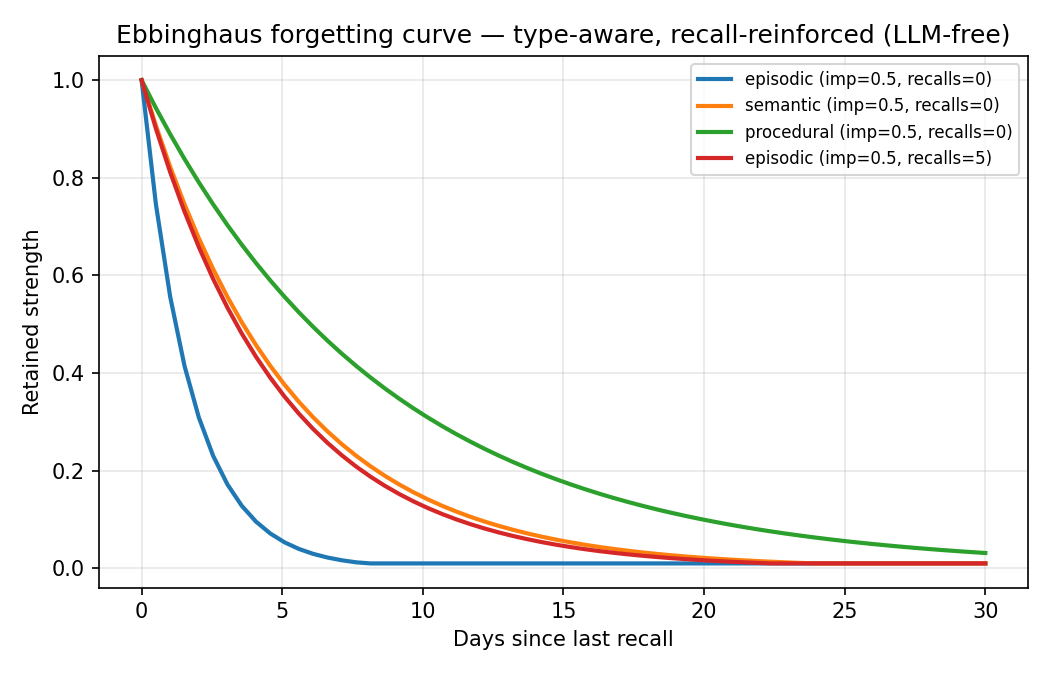
\includegraphics[width=0.74\linewidth]{figures/fig1_forgetting.png}
\caption{On-device forgetting dynamics by memory type. Episodic appears twice
deliberately: once never recalled (fastest fade) and once recalled $5\times$,
showing that recall reinforcement flattens the curve. Type stability
multipliers: episodic $1\times$, semantic $3\times$, procedural $5\times$;
recall raises stability via $\ln(2+\text{access\_count})$.}
\label{fig:forget}
\end{figure}

\subsection{Self-knowledge is operational}\label{sec:exp-selfknow}
We fix a memory's query relevance and sweep its stored confidence across each
epistemic status, measuring the resulting composite retrieval score with the
modifier \textbf{on} versus a baseline with it \textbf{off} (relevance only,
score $0.5945$). Figure~\ref{fig:rank} shows the score rising with confidence and
the \status{uncertain}/\status{contradicted} curves sitting strictly below
\status{verified}/\status{inferred} (at confidence $1.0$: verified $0.5945$,
uncertain $0.5053$, contradicted $0.2972$). Table~\ref{tab:modifier} reports the
modifier $\mathrm{epi}(m)$ itself, independent of relevance.

\begin{figure}[h]
\centering
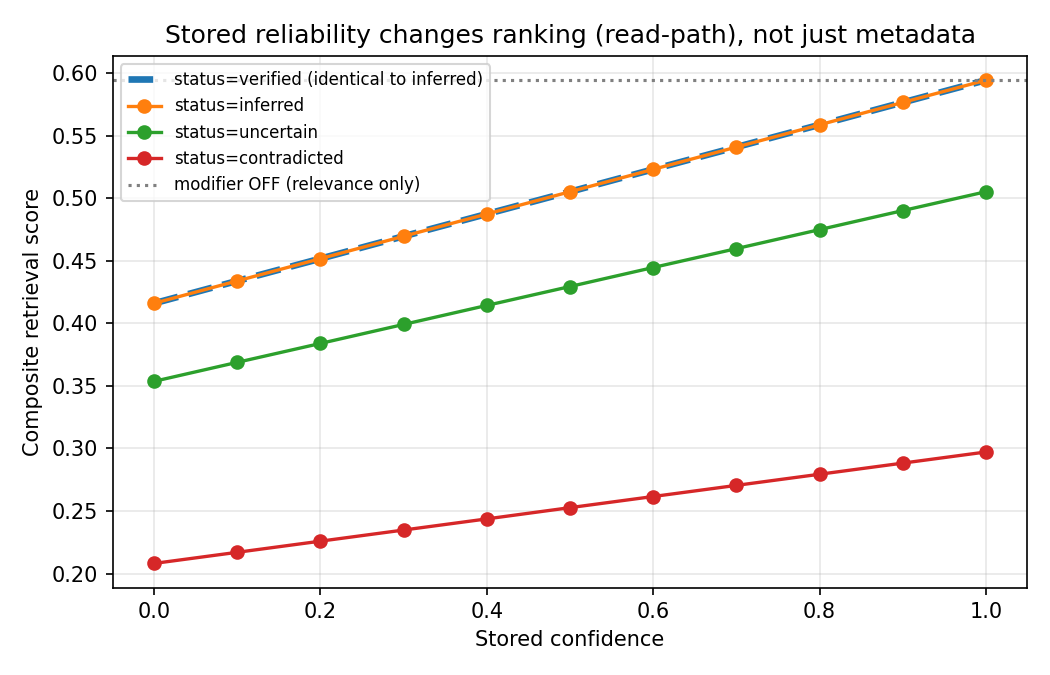
\includegraphics[width=0.74\linewidth]{figures/fig2_confidence_ranking_v2.png}
\caption{Composite retrieval score at fixed relevance as stored confidence varies,
per epistemic status. The \status{verified} curve (dashed) coincides exactly with
\status{inferred}, since both carry status penalty $1.0$. Identical relevance,
different reliability, different ranking---the concrete sense in which
self-knowledge is operational.}
\label{fig:rank}
\end{figure}

\begin{table}[h]
\centering\small
\caption{The epistemic modifier $\mathrm{epi}(m)$ of Eq.~\eqref{eq:modifier},
by status and confidence.}
\label{tab:modifier}
\begin{tabular}{lccc}
\toprule
status & $\kappa=0.0$ & $\kappa=0.5$ & $\kappa=1.0$ \\
\midrule
\status{verified}      & 0.70 & 0.85 & 1.00 \\
\status{inferred}      & 0.70 & 0.85 & 1.00 \\
\status{uncertain}     & 0.595 & 0.722 & 0.85 \\
\status{contradicted}  & 0.35 & 0.425 & 0.50 \\
\bottomrule
\end{tabular}
\end{table}

\subsection{End-to-end contradiction handling}\label{sec:exp-contra}
We store a fact, then a contradicting update, and query for it. The old memory's
status becomes \status{contradicted} (confidence floored to $0.3$, marked
non-current), the new memory \emph{is} returned by recall while the stale one is
\emph{suppressed} (recall returns new${}={}$true, returns old${}={}$false), and
the supersession link is recorded for audit.

\subsection{Self-audit precision}\label{sec:exp-lint}
On a fresh store seeded with healthy filler plus \emph{planted} issues,
\code{lint} recovers them (Table~\ref{tab:lint}). Planted issues are
controlled---explicit \status{contradicts} links, back-dated never-accessed
memories, and an embedding-identical near-duplicate---so this measures detection
mechanics, not real-world prevalence.

\begin{table}[h]
\centering\small
\caption{Self-audit detection on planted issues (\code{lint}).}
\label{tab:lint}
\begin{tabular}{lcc}
\toprule
issue type & planted & caught \\
\midrule
contradiction & 1 & 1 \\
stale         & 3 & 3 \\
duplicate     & 1 & 1 \\
\bottomrule
\end{tabular}
\end{table}

\subsection{Latency and footprint}\label{sec:exp-latency}
Storing $400$ memories and issuing $80$ recalls on a laptop (local embeddings
$+$ local cross-encoder reranker, no LLM): recall latency
$\text{p50}=78.6$\,ms, $\text{p95}=190.5$\,ms (mean $95.1$\,ms); store
throughput $27.8$\,ms/memory; on-disk footprint ${\approx}4.4$\,MB (SQLite)
$+\,{\approx}4.8$\,MB (FAISS). The system is comfortably interactive on consumer
hardware with no server and no network.

\subsection{Does the epistemic signal help? A fair ablation}\label{sec:exp-fair}
The preceding experiments show the epistemic modifier \emph{fires}; this one
tests whether it \emph{helps}, isolating its contribution from the mere presence
of an abstention option. We hold the system, the store, and the abstention
mechanism fixed and toggle \emph{only} the modifier: a \textbf{baseline} ranks
with \code{use\_epistemic=False} and an \textbf{epistemic} policy with
\code{use\_epistemic=True}; both then abstain when the top composite score falls
below a threshold $\theta$, which we sweep for each so neither is advantaged by a
hand-picked value. The store holds $15$ deliberately diverse facts per class
(verified intact: $0$ supersession events, $30/30$ memories current, so there is
no duplicate-collapse artifact): \emph{trusted} (current, verified---should
answer), \emph{low-trust} (current, but marked \status{contradicted}/
\status{uncertain} with low confidence---should abstain), and \emph{absent}
(nothing relevant stored---should abstain). Correctness is value-based,
independent of which memory is retrieved.

The decisive subset is \emph{low-trust}, where a still-relevant memory scores
high on pure relevance: the baseline confidently surfaces it, whereas the
epistemic modifier multiplies its score by the status penalty and confidence
floor, pushing it below $\theta$. Table~\ref{tab:fair} reports a matched
operating point ($\theta{=}0.60$, where \emph{both} policies retain $100\%$
answerable coverage); Figure~\ref{fig:fair-sweep} shows the full sweep and
Figure~\ref{fig:fair-lowtrust} the low-trust subset.

\begin{table}[h]
\centering\small
\caption{Fair ablation: same store, only the epistemic modifier toggled,
abstention threshold swept, reported at a matched operating point
($\theta{=}0.60$; both policies at $100\%$ answerable coverage; $n{=}15$ per
class; on-device, LLM-free). Lower is better for confident-wrong rates.}
\label{tab:fair}
\begin{tabular}{lcc}
\toprule
Metric & Baseline (relevance-only) & Epistemic \\
\midrule
Answerable accuracy ($\uparrow$)         & 100\% & 100\% \\
Low-trust confident-wrong ($\downarrow$) & 33.3\% & 0.0\% \\
Absent confident-wrong ($\downarrow$)    & 0.0\% & 0.0\% \\
Overall confident-wrong ($\downarrow$)   & 11.1\% & 0.0\% \\
Abstention F1 ($\uparrow$)               & 0.91 & 1.00 \\
\bottomrule
\end{tabular}
\end{table}

\begin{figure}[h]
\centering
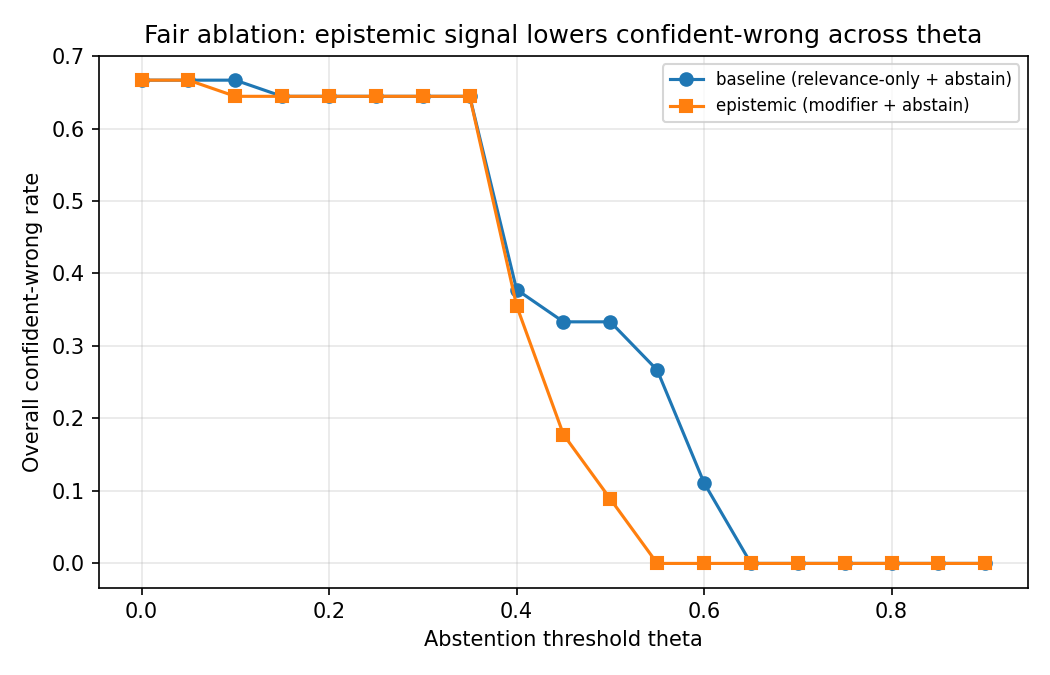
\includegraphics[width=0.70\linewidth]{fair_eval/fig_sweep_selfcontained.png}
\caption{Confident-wrong rate versus the abstention threshold $\theta$, for the
relevance-only baseline and the epistemic policy on the identical store. The
epistemic curve sits at or below the baseline throughout: the same retrieval,
with stored reliability folded in, makes fewer confident errors.}
\label{fig:fair-sweep}
\end{figure}

\begin{figure}[h]
\centering
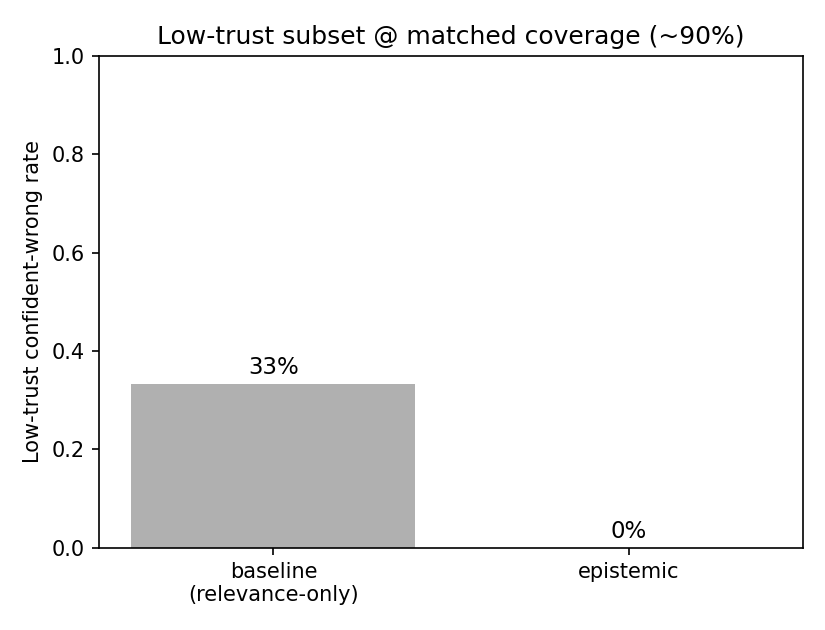
\includegraphics[width=0.52\linewidth]{fair_eval/fig_lowtrust_selfcontained.png}
\caption{Low-trust subset at the matched operating point ($\theta{=}0.60$,
$100\%$ answerable coverage). The baseline confidently answers from memories the
system itself marked contradicted/uncertain ($33.3\%$); the epistemic policy
demotes them below threshold and abstains ($0\%$).}
\label{fig:fair-lowtrust}
\end{figure}

\paragraph{Takeaway.}
At an identical threshold and identical $100\%$ answerable coverage, folding
stored reliability into ranking cuts low-trust confident-wrong answers from
$33.3\%$ to $0\%$ (overall confident-wrong $11.1\%\!\rightarrow\!0\%$; abstention
F1 $0.91\!\rightarrow\!1.00$). The effect is robust across the
coverage-preserving band, not a single-$\theta$ artifact: the epistemic policy
reaches $0\%$ low-trust confident-wrong by $\theta{=}0.55$ while the baseline is
still at $80\%$ there. Because both policies share the same store and abstention
rule, the gain is attributable to the epistemic signal itself, not to having an
abstention option. The store is small ($n{=}15$ per class) and the low-trust
conditions are constructed, so this isolates the read-path mechanism rather than
demonstrating field prevalence (\S\ref{sec:limits}).

% =====================================================================
\section{Proposed Extensions}\label{sec:extensions}
% =====================================================================
The epistemic state above also enables capabilities we specify but do not yet
fully evaluate; we describe them precisely and release harnesses so they can be
measured. (Grounded abstention---the most developed of these---is evaluated in
\S\ref{sec:exp-fair}.)

\paragraph{Belief propagation through consolidation.}
A memory derived from others (consolidation or synthesis) should inherit the
\emph{most conservative} status of its sources and a confidence that is a
function of source agreement, with a \status{derived} provenance edge. Provenance
for derived memories is recorded today; principled status/confidence propagation
through the consolidation engine is specified here and is partially realized.

\paragraph{External benchmarking.}
Our experiments characterize mechanics, not comparative accuracy. We release a
benchmark runner that ingests each LongMemEval-S~\cite{longmemeval}
chat history into Memory Layer, answers through the abstention policy, and emits
predictions in the benchmark's format for its official judge---reporting overall
accuracy and, in particular, the \emph{knowledge-update} and \emph{abstention}
slices, where an epistemic memory should help most. This is our recommended next
step.

% =====================================================================
\section{Limitations}\label{sec:limits}
% =====================================================================
\begin{itemize}[leftmargin=1.4em]
  \item \textbf{No competitive QA benchmark yet.} We report no
  LoCoMo/LongMemEval accuracy or head-to-head comparison against Mem0/Zep/Letta;
  the runner exists but full, baseline-matched runs have not been done, so we
  make no accuracy-superiority claim.
  \item \textbf{Controlled, partly synthetic demonstrations.}
  \S\ref{sec:exp-contra}--\ref{sec:exp-fair} use small, constructed inputs to
  isolate mechanics, not field prevalence: in particular the fair ablation uses
  $n{=}15$ facts per class with constructed low-trust statuses, and its effect
  lives in a fairly narrow (though internally robust) $\theta$ band.
  \item \textbf{Confidence is heuristic, not calibrated.} The priors of
  Eq.~\eqref{eq:formation} are hand-set; we do not show they match empirical
  correctness (a reliability-diagram/ECE study is future work).
  \item \textbf{Consolidation synthesis needs an LLM.} The fully LLM-free path is
  extractive; abstractive synthesis benefits from a (local) LLM.
  \item \textbf{Hand-set thresholds.} The duplicate cutoff ($0.95$), staleness
  window ($14$ days), and modifier constants ($W_{\!f}$, the penalties) are not
  tuned or learned.
  \item \textbf{Single machine.} Multi-user/distributed behavior is out of scope.
\end{itemize}

% =====================================================================
\section{Conclusion}
% =====================================================================
We presented a memory layer that pushes the \emph{local, LLM-free} constraint as
far as it will go and makes a memory's self-knowledge operational: reliability
governs retrieval, and the store audits itself, all on-device and characterized
on consumer hardware. The contribution is integration and operationalization, not
a new algorithm, and we characterize rather than claim to beat a benchmark. The
unifying view is that contradiction handling, knowledge updates, provenance,
self-audit, and abstention are one thing seen from different angles: operations
on \emph{belief}. We release all code and reproduction scripts, and identify
external long-horizon evaluation as the clear next step.

\section*{Reproducibility and Availability}
The system, the maintenance loop, the epistemic modifier, the self-audit, and a
test suite of 147 unit and integration tests are released as open source,
together with scripts that regenerate every figure and number in this paper
(the characterization suite for \S\ref{sec:exp-forget}--\ref{sec:exp-latency},
the fair-ablation script for \S\ref{sec:exp-fair}, and a runner for the
LongMemEval benchmark). The on-device experiments are deterministic and require
no API key. The repository URL will accompany the public release.

% =====================================================================
\begin{thebibliography}{99}
\small

\bibitem{memgpt} C. Packer, S. Wooders, K. Lin, V. Fang, S. G. Patil, I. Stoica,
and J. E. Gonzalez. \emph{MemGPT: Towards LLMs as Operating Systems}.
arXiv:2310.08560, 2023.

\bibitem{mem0} P. Chhikara, D. Khant, S. Aryan, T. Singh, and D. Yadav.
\emph{Mem0: Building Production-Ready AI Agents with Scalable Long-Term Memory}.
arXiv:2504.19413, 2025.

\bibitem{zep} P. Rasmussen, P. Paliychuk, T. Beauvais, J. Ryan, and D. Chalef.
\emph{Zep: A Temporal Knowledge Graph Architecture for Agent Memory}.
arXiv:2501.13956, 2025.

\bibitem{amem} W. Xu, Z. Liang, K. Mei, H. Gao, J. Tan, and Y. Zhang.
\emph{A-MEM: Agentic Memory for LLM Agents}. arXiv:2502.12110, 2025.

\bibitem{memorybank} W. Zhong, L. Guo, Q. Gao, H. Ye, and Y. Wang.
\emph{MemoryBank: Enhancing Large Language Models with Long-Term Memory}.
In \emph{AAAI}, 2024. arXiv:2305.10250.

\bibitem{generativeagents} J. S. Park, J. C. O'Brien, C. J. Cai, M. R. Morris,
P. Liang, and M. S. Bernstein. \emph{Generative Agents: Interactive Simulacra of
Human Behavior}. In \emph{UIST}, 2023. arXiv:2304.03442.

\bibitem{rag} P. Lewis et al. \emph{Retrieval-Augmented Generation for
Knowledge-Intensive NLP Tasks}. In \emph{NeurIPS}, 2020. arXiv:2005.11401.

\bibitem{graphrag} D. Edge, H. Trinh, N. Cheng, et al. \emph{From Local to
Global: A Graph RAG Approach to Query-Focused Summarization}. arXiv:2404.16130,
2024.

\bibitem{doyle} J. Doyle. \emph{A Truth Maintenance System}. Artificial
Intelligence, 12(3):231--272, 1979.

\bibitem{atms} J. de Kleer. \emph{An Assumption-based TMS}. Artificial
Intelligence, 28(2):127--162, 1986.

\bibitem{agm} C. E. Alchourr\'on, P. G\"ardenfors, and D. Makinson. \emph{On the
Logic of Theory Change: Partial Meet Contraction and Revision Functions}.
Journal of Symbolic Logic, 50(2):510--530, 1985.

\bibitem{provenance} P. Buneman, S. Khanna, and W.-C. Tan. \emph{Why and Where:
A Characterization of Data Provenance}. In \emph{ICDT}, 2001.

\bibitem{calibration} C. Guo, G. Pleiss, Y. Sun, and K. Q. Weinberger. \emph{On
Calibration of Modern Neural Networks}. In \emph{ICML}, 2017.

\bibitem{selective} Y. Geifman and R. El-Yaniv. \emph{Selective Classification
for Deep Neural Networks}. In \emph{NeurIPS}, 2017.

\bibitem{longmemeval} D. Wu et al. \emph{LongMemEval: Benchmarking Chat
Assistants on Long-Term Interactive Memory}. In \emph{ICLR}, 2025.
arXiv:2410.10813.

\bibitem{memx} L. Sun. \emph{MemX: A Local-First Long-Term Memory System for AI
Assistants}. arXiv:2603.16171, 2026.

\bibitem{hindsight} Latimer et al. \emph{Hindsight is 20/20: Building Agent
Memory that Retains, Recalls, and Reflects}. arXiv:2512.12818, 2025.

\bibitem{governed} H. Taheri. \emph{Governed Memory: A Production Architecture
for Multi-Agent Workflows}. arXiv:2603.17787, 2026.

\bibitem{toki} Z. Wang. \emph{TOKI: A Bitemporal Operator Algebra for
Contradiction Resolution in LLM-Agent Persistent Memory}. arXiv:2606.06240,
2026.

\bibitem{eywa} R. Joshi. \emph{Eywa: Provenance-Grounded Long-Term Memory for
AI Agents}. arXiv:2605.30771, 2026.

\bibitem{memaudit} Z. Tan, Y. Yao, H. Jin, W. Yu, G. Wang, M. Fan, et al.
\emph{MemAudit: Post-hoc Auditing of Poisoned Agent Memory via Causal
Attribution and Structural Anomaly Detection}. arXiv:2605.23723, 2026.

\bibitem{locomo} A. Maharana, D.-H. Lee, S. Tulyakov, M. Bansal, F. Barbieri,
and Y. Fang. \emph{Evaluating Very Long-Term Conversational Memory of LLM
Agents (LoCoMo)}. In \emph{ACL}, 2024. arXiv:2402.17753.

\end{thebibliography}

\end{document}
